\section{\textit{SuperSet}, \textit{SuperSetProducer}, és \textit{SuperSetConsumer}}

    A fejezet címében szereplő három komponenst, amelyek az \textbf{\ref{fig:component-sets}. ábrán} láthatóak,
    egyszerre tekintjük át. Ennek egyszerű oka a komponensek működése nagyon hasonló. Fő szerepük a munka hatékony
    felosztása az elérhető hardvereken. A hasonlóság okán közös ősosztályból örökölnek ez a \textit{SuperSetBase}. Ez
    az osztály kezeli a közös parancssori argumentumokat, beállítja a munkakönyvtárat, és példányt készít a
    \textit{ConfigManager} objektumból.

    Ezek a komponensek kapják meg bemenetként a teszt csomagokat, majd osztják szét azokat, végül aggregálják az
    eredményeket, így tekinthetünk rájuk úgyis mint egy fordítóprogram meghajtó részére. Egyszerűen kifejezve a
    tesztfuttatás menetét felügyelik, úgy ahogyan egy fordítóprogram meghajtó felügyeli a fordítás menetét.

    A \textit{SuperSet} komponens, ahogy azt a~\ref{sec:project-structure} fejezetben említettem, a lokális futtatást
    oldaja meg. A \textit{SuperSetConsumer} (röviden \textit{Consumer}) pedig, az elosztott működésben a kliens oldalt
    valósítja meg.

    Miután a \textit{ConfigManager} (\ref{chp:config-manager}.\ fejezet) előállítja az összes teszt csomag objektumot,
    és kiszámolja azoknak a mátrixait illetve megszorításait, a \textit{SuperSet} szétosztja munkafolyamatokra a
    csomagokban található egyes tesz eseteket.

    \subsection{A munkafolyamatok}

        A \textit{SuperSet} esetében három, a \textit{SuperSetConsumer} esetében kettő a \textit{SuperSetProducer}
        esetében pedig egy munkafolyamat jön létre. A munkafolyamatokat az \textbf{\ref{fig:superset-workflows}.
        táblázat mutatja}.

        \begin{table}[ht]
            \centering
            \begin{tabular}{lccc}
                \toprule
                \diagbox{Work}{Comp.} & \textit{SuperSet}   & \textit{Consumer}   & \textit{Producer}   \\
                \midrule
                Create job            & {\dbfont\textbf{✓}} & {\dbfont\textbf{✓}} &                     \\
                Do job                & {\dbfont\textbf{✓}} & {\dbfont\textbf{✓}} &                     \\
                Report job result     & {\dbfont\textbf{✓}} &                     & {\dbfont\textbf{✓}} \\
                \bottomrule

            \end{tabular}
            \caption{\label{fig:superset-workflows} A munkafolyamatok komponensenként}
        \end{table}

        \noindent
        Az \textbf{\ref{fig:superset-workflows}.\ táblázatban} látott munkafolyamatok az alábbi módon működnek:

        \begin{itemize}
            \item Munka létrehozás \textit{(Create job)}: A beérkező tesztcsomagokból és azokra vonatkozó
                  konfigurációkból munkákat tesz egy \textbf{FIFO sorba}.
            \item Munkavégzés \textit{(Do job)}: A \textbf{FIFO sorból} kivesz egy munka elemet majd végre hajtja a
                  fordítóprogramhoz implementált \textit{SystemUnderTest} bővítménnyel.
            \item Eredmény aggregálás \textit{(Report job result)}: az eredmények adatbázisba mentése.
        \end{itemize}

        \pagebreak
        A munkafolyamatok a Python nyelv standard aszinkron eseményciklusában futnak
        (\textit{asyncio}~\cite{pythonasyncio}).

        Több alternatívát is megvizsgáltam. A hagyományos szál kezelés a Python nyelvben lassú a \textit{Global
        Interpreter Lock} miatt.

        Egy másik alternatíva a \textit{multiprocessing~\cite{pythonmultiprocessing}} modul használata, azonban ez a
        modul a számítás igényes feladatokon hoz jó teljesítményt, a keretrendszer viszont legtöbb idejét \textit{I/O}
        folyamatokra várással tölti. A tesztelt fordítóprogram kimenetére vár.

        Ezért az aszinkron párhuzamosítás bizonyult a legjobb megoldásnak.

        \subsubsection{A munkafolyamat sor}

            A munkafolyamat sor egy \textbf{FIFO sor}.

            Viszonylag könnyen belátható, hogy ha a munkafolyamatok első két lépést, azaz a létrehozást és a futtatást
            szekvenciálisan hajtanánk végre, akkor nem lenne szükség a \textit{munkafolyamat sorra}. Elég lenne egy
            egyszerű algoritmust alkalmazva létrehozni egy \textbf{Szemafort}, a hardverünkön elérhető mennyiségű CPU
            mag számmal.

            Azonban a munkafolyamatok létrehozása is \textit{I/O} költséges művelet, mivel a teszteseteket be kell
            olvasni lemezről, valamint külön-külön mappákat kell létrehozni ahová a fordítóprogram a kimenetét
            generálja, így elkerülhető a fájlnév ütközés.

            Ez az \textit{I/O} költség indokolja a \textit{munkafolyamat sor} létét. Máskülönben, gyorsan futó
            tesztesetek esetén előfordulhatna, hogy nincs munka mert az \textit{I/O} műveletekre várunk, tehát a
            folyamatunk éhezne!

            Ugyanakkor azt is lehet látni, hogy a \textit{munkafolyamat sorhoz} való hozzáférést védeni kell egy
            \textbf{Mutexel}. Ennek a mutexnek a megszerzése \textbf{zárolási versenyhez} vezethet ami ugyanúgy
            éhezteti a folyamatunkat.

            Ennek megoldására azt a heurisztikát választottam, hogy egy adott tesztcsomag egy adott konfigurációját
            mindig egyszerre adja hozzá a munka létrehozó folyamat a sorhoz. Így a létrehozó folyamatok
            nagyságrendekkel kevesebb időt töltenek a sor zárolásával, mint a futtató folyamatok.

            Természetesen ez a heurisztika arra a megfigyelésre támaszkodik, hogy egy tesztcsomaghoz sok teszteset
            tartozik, és/vagy sok konfiguráció, így a végső tesztesetek száma legalább egy-két nagyságrenddel több mint
            a tesztcsomagok száma. Ha ez nem teljesül, esetleg még a nagyságrendbeli viszony is megfordul, akkor a
            futtatás lassabb mint az alternatív \textit{Szemafort} használó implementáció.

            \pagebreak
        \subsubsection{Az eredmény aggregálás}

            Az eredmények aggregálása implementációját tekintve különbözik az elosztott és a lokális futtatások között.

            A \textit{SuperSet} lokális komponens esetében a lefuttatott tesztesetek eredményi szintén egy \textbf{FIFO
            sorba} kerülnek. Mivel az aggregáló folyamatból csak egy fut így nem kell aggódni, hogy \textit{zárolási
            verseny} lépne fel. Az aggregáló folyamat csak akkor indul el ha már minden munka elő lett készítve.

            A \textit{SuperSetProducer} elosztott szerver oldali komponens esetében a lefuttatott eredményeket a
            szerver tömbösítve egy tesztcsomag egy konfigurációjánként kapja vissza.

            Az implementációban közös, hogy mindkét esetben az eredmények egy \textit{SQLite} alapú adatbázisban
            lesznek elérhetőek. Jogosan merül fel a kérdés, hogy egy egyszerű leírónyelv fájl kimenet is megfelelő
            lehet.

            Azonban az \textit{SQLite} adatbázisnak több előnye is van. Először is \textit{SQL} nyelven írható hozzá
            lekérdezés így könnyen lehet szűrni az eredmények között. Továbbá az adatbázis egy tömörebb bináris
            formátumban tárolja az adatot, ez segít az eredmények könnyebb tárolásában. Ennél viszont sokkal fontosabb
            tulajdonsága, hogy hozzáfűzni egy új eredményt egy nagy adatbázishoz közel ugyanannyi idő mint egy üreshez.
            Ez fájlok esetében nem mondható el ahol az egész fájlt, vagy az azt reprezentáló adatstruktúrát memóriában
            kell tartani. Mivel egy futás eredmény több \textbf{megabájt} is lehet így az adatbázisba írás sokkal
            gyorsabb.

    \subsection{A szerver-kliens kommunikáció}

        Az elosztott működés során szükség van egy protokollra és egy állapot megosztásra a szerver és a kliensek
        között.

        A szerver mindaddig fenntartja a kapcsolatot a kliensekkel ameddig az \textbf{összes} kliens be nem fejezi a
        futást. Ennek az az oka, hogy ameddig nem lett minden teszt lefuttatva, akkor egy váratlan esemény
        bekövetkezésekor a kiosztott tesztek elveszhetnek. Ilyen kliens oldali váratlan esemény lehet egy futás során
        bekövetkező összeomlás, vagy egy hálózati kapcsolati hiba.

        Ha egy kliens váratlan módon lecsatlakozik a szerverről, akkor a szerver az annak a kliensnek küldött legutóbbi
        tesztcsomagokat újra kiosztja egy másik kliensnek. Ezért a kliensprogramok ha egyszer csatlakoztak, akkor
        egészen addig várnak ameddig a szerver nem terminál.

        \pagebreak
        \subsubsection{A szerver-kliens protokoll}

            A szerver a kliensekkel egy jól meghatározott protokollon keresztül kommunikál, amelyet kifejezetten az
            alkalmazás igényeihez terveztem. A kommunikáció egy \textit{WebSocket}~\cite{websocket} csatornán keresztül
            történik. A protokoll struktúráját az alábbi \textbf{\ref{fig:protocol-buffer}. ábra} szemlélteti.

            \begin{figure}[ht]
                \centering
                \hrule
                \vspace{1mm}
                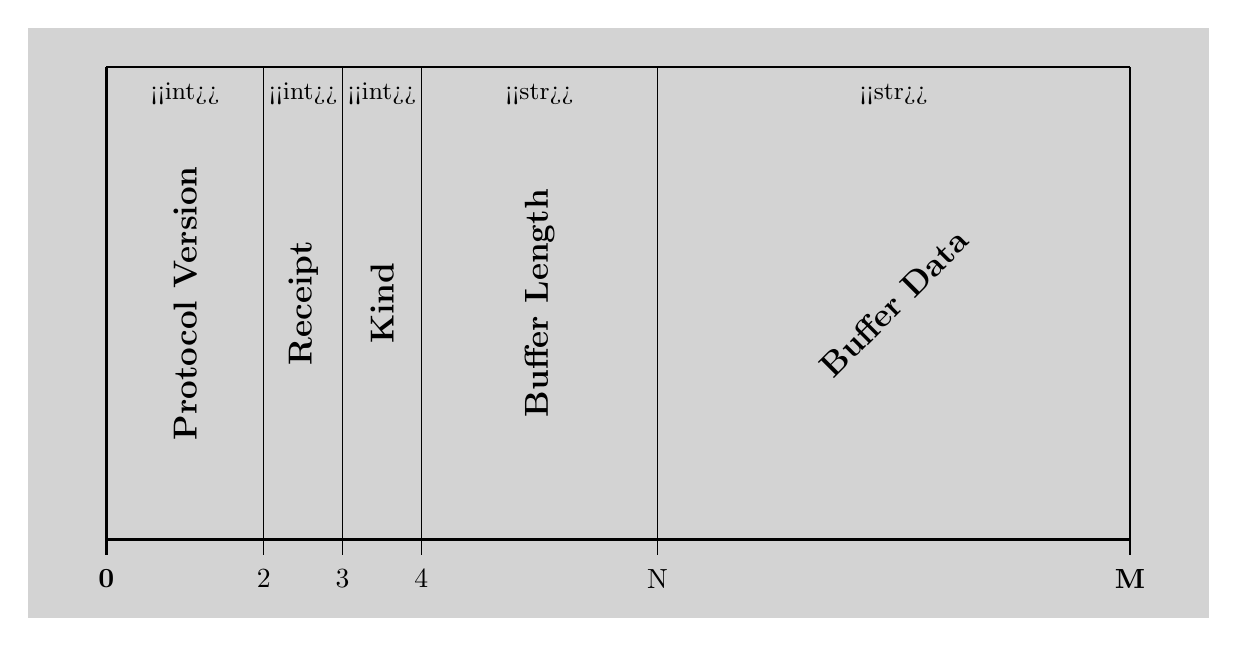
\begin{tikzpicture}
                    % Outline
                    \fill[LightGray] (-8,4.5) rectangle (7,-3);

                    % Buffer outlines
                    \draw[thick] (-7, 4) -- (6, 4);
                    \draw[thick] (-7, -2) -- (6, -2);
                    \draw[thick] (-7, 4) -- (-7, -2.2);
                    \draw[thick] (6,4) -- (6, -2.2);

                    % Buffer start, end size
                    \node at (-7, -2.5) {\textbf{0}};
                    \node at (6, -2.5) {\textbf{M}};

                    % Segment lines
                    \draw (-5, 4) -- (-5, -2.2);
                    \draw (-4, 4) -- (-4, -2.2);
                    \draw (-3, 4) -- (-3, -2.2);
                    \draw (0, 4) -- (0, -2.2);

                    % Segment size
                    \node at (-5, -2.5) {2};
                    \node at (-4, -2.5) {3};
                    \node at (-3, -2.5) {4};
                    \node at (0, -2.5) {N};

                    % Segment text
                    \node at (-6, 1) {\rotatebox{90}{\large\textbf{Protocol Version}}};
                    \node at (-4.5, 1) {\rotatebox{90}{\large\textbf{Receipt}}};
                    \node at (-3.5, 1) {\rotatebox{90}{\large\textbf{Kind}}};
                    \node at (-1.5, 1) {\rotatebox{90}{\large\textbf{Buffer Length}}};
                    \node at (3, 1) {\rotatebox{45}{\large\textbf{Buffer Data}}};

                    \node at (-6, 3.66) {\small<<int>>};
                    \node at (-4.5, 3.66) {\small<<int>>};
                    \node at (-3.5, 3.66) {\small<<int>>};
                    \node at (-1.5, 3.66) {\small<<str>>};
                    \node at (3, 3.66) {\small<<str>>};
                \end{tikzpicture}
                \vspace{-3mm}
                \hrule
                \caption{\label{fig:protocol-buffer} A protokoll csomag bájt mérete}
            \end{figure}

            A csomag a hálózati kommunikáció szabványos módja szerint, \textit{\foreignlanguage{american}{big-endian}}
            bájtsorrendben van lekódolva. A csomagban lévő típusok egész számok és sztringek. A sztringek
            \textit{UTF-8} kódoltak így nem érintettek a bájt sorrend problémában, mivel ez a kódolás egy bájtonként
            olvassa a puffert.

            A protokoll csomag először \emph{2 bájtot} küld amiben a protokoll verziója van. Ez biztonsági okokbólí
            szükséges. Ha a jövőben változtatni szeretnék a protokoll struktúráján akkor azt könnyen megtehetem, mert
            ha a verziók nem egyeznek akkor a kapcsolat nem épül fel.

            A következő bájt a protokoll állapotát visszajelző nyugta. A küldő mindig \textit{0} bájtot küld, a fogadó
            pedig mindig \textit{1} bájtal válaszol. A legfelső \textit{255} bájt foglalt általános hiba
            visszajelzésre.

            A következő bájt az üzenet típusát azonosítja amely a következők egyike lehet:

            \begin{itemize}
                \item \textit{*InitialData}: A kliens küldi a szervernek csatlakozáskor. Tartalmazza a kliens őforrásait
                      \textit{(CPU magok száma)}, és a \textit{host nevét}.
                \item \textit{ReqWork}: A kliens küldi amikor készen áll a teszt futtatásra.
                \item \textit{*ClientConfig}: A szerver küldi a kliensnek, hogy milyen konfigurációs fájlt töltsön be.
                \item \textit{*TestData}: A szerver küldi a kliensnek. Ez a csomag tartalmaz valamennyi tesztcsomagot.
                \item \textit{*Result}: A kliens küldi a szervernek. Ez a csomag tartalmazza a legutóbbi tesztcsomagok
                      eredményeit.
                \item \textit{Disconnect}: A szerver küldi a kliensnek ha lecsatlakozhat. A szerver zárás előtt kerül
                      kiküldésre minden kliensnek.
            \end{itemize}

            A következő bájtokat a protokoll egy \textit{'\textbackslash{}n'} karakterig olvassa. Ha nullánál több
            bájtot olvasott, akkor annak tartalmát egy előjel nélküli egész számként kezeli ami a következő pufferben
            lévő adat mennyiségét jelzi. Az előző listában \textit{*-al} megjelölt üzenet típusokhoz tartozik adat,
            azaz nem üres a \textit{Buffer Data}.

            Végül a protokoll annyi bájtot olvas amennyi az előjel nélküli egész szám értéke. Ez az adat mindig
            \textit{JSON}~\cite{json} formátumban érkezik.

        \subsubsection{A szerver kontextus}

            A szerver alkalmazás egy kontextusban tárolja az összes csatlakozott klienst. Így ha egy kliens kiesik
            valamilyen nem várt hiba okán, akkor azonnal át tudja irányítani a munkát egy másik kliensre, ha az éppen
            nem dolgozik.

            A szerver az előre elkészített tesztcsomagokból álló üzeneteket egy sorban tárolja. Amikor elküld ebből a
            sorból valamennyi üzenetet akkor egy \textit{kontextus kezelőbe} lép. Ez a \textit{kontextus kezelő}
            feljegyzi a szerver kontextusába, hogy az adott kliens éppen dolgozik és megvárja az eredményeket. Ha ez
            nem sikerül a kliensnek akkor a \textit{kontextus kezelő} visszarakja a sorba a kivett üzeneteket. Ezt a
            viselkedést a \textbf{\ref{fig:client-ctx-handler}. ábra} mutatja be.

            \begin{figure}[ht]
                \centering
                \begin{minted}{python}
@asynccontextmanager
async def begin_client_work(
    ctx: "Context",
    client: Client,
    test_batch: Collection[TestCasePackage],
) -> AsyncIterator[None]:
    await ctx.set_client_working(client, True)  # Client begins work
    try:
        yield  # wait for client to finish
    except ProtocolError:
        # Client failed somehow, re-adding tests to the Queue
        await ctx.add_tests(test_batch)
    finally:
        await ctx.set_client_working(client, False)  # Client ends work
                \end{minted}
                \caption{\label{fig:client-ctx-handler} A kliens állapotát, felügyelő \textit{kontextus kezelő}}
            \end{figure}

        \subsubsection{Összegzés}

            A protokoll mögötti tervezési konstrukció egy hibatűrő, és minimális rendszert alkot. A kommunikációra
            tudatosan nem a \textit{HTTP}~\cite{http} protokollt választottam mert az sok fölösleges plusz
            információval rendelekezik, a megoldott problémával összevetve. Az implementált protokoll tökéletesen
            modellezi az elosztott keretrendszer invarianciáit, és minimális adatot küld.
